\documentclass{beamer}
\usetheme{Warsaw}
\useinnertheme{circles}
\useoutertheme[subsection=false]{smoothbars}
\usepackage[utf8x]{inputenc}
\usepackage[czech]{babel}
\usepackage[T1]{fontenc}
\usepackage{listings}
\usepackage{tikz}
\lstset{basicstyle=\tiny\ttfamily}
\logo{
\includegraphics[height=0.5cm]{brmlab.pdf}}

\begin{document}

\AtBeginSection[]
{
  \begin{frame}
    \frametitle{Outline}
    \tableofcontents[currentsection]
  \end{frame}
}

\title{brmiversity: Umělá inteligence \\ a teoretická informatika}
\subtitle{Přednáška č. 9}
\author{Petr Baudiš $\langle${\tt pasky@ucw.cz}$\rangle$}
\institute{
	brmlab 2011\\
	\vskip 1ex
	\pgfdeclareimage[height=4ex]{ccbysa}{by-sa.pdf}
	\pgfuseimage{ccbysa}
}
\date{}
\frame{\titlepage}

\section{Umělá inteligence}

\subsection{}
\begin{frame}{Strojové učení}
\begin{center}
Učící se agent: Datový vstup a výstup, rozhodovací problém, užitková funkce
\vskip 3ex
\begin{block}{Máme trénovací množinu}
\begin{itemize}
\item Učení s učitelem vs. bez učitele
\item Rozpoznávání vs. samoorganizace
\end{itemize}
\end{block}
\begin{block}{Nemáme trénovací množinu}
\begin{itemize}
\item Exploration---exploitation dilemma
\item Zpětnovazebné učení
\end{itemize}
\end{block}
\end{center}
\end{frame}

\subsection{}
\begin{frame}{Strojové učení nad daty}
\begin{center}
Dnes: Máme trénovací a testovací data, hledáme {\em hypotézu}. \\
Chceme řešit buď {\em klasifikační} nebo {\em regresní} úlohy. \\
Parametrické vs. reprezentační metody.
\end{center}
\end{frame}

\subsection{}
\begin{frame}{Strojové učení nad daty}
\begin{block}{Učení s učitelem}
\begin{itemize}
\item Prohledávání prostoru verzí
\vskip 1ex
\item {\bf Rozhodovací stromy}
\item {\bf Bayesovské učení}
\item Částicové filtry
\vskip 1ex
\item Neuronové sítě
\item {\bf Support Vector Machines}
\end{itemize}
\end{block}
\begin{block}{Učení bez učitele}
\begin{itemize}
\item Karuhnenova-Loèveho transformace (PCA)
\item {\bf Clusterování}
\item Kohonenovy mapy
\item Lineární regrese
\end{itemize}
\end{block}
\end{frame}

\subsection{}
\begin{frame}{Rozhodovací stromy}
\begin{itemize}
\item Mějme databázi $\vec D$ jedinců; jedinec je popsán příznakovým vektorem atributů $\vec t$; jedinec patří do třídy $c$
\item Rozhodovací strom definuje posloupnost dotazů na atributy pro určení třídy
\item Bankovní klienti, expertní systémy
\item Konstrukce: Algoritmus ID3 maximalizující informační zisk
\item {\em Informační entropie} $H = -\sum_a (p_a \log_2 p_a)$ ($a$ je konkr. hodnota konkr. atributu)
\item Entropie je míra překvapení v množině, chceme co největší redukci překvapení
\item Výběr atributů nebo malý dataset: Pozor na přeučení
\end{itemize}
\end{frame}

\subsection{}
\begin{frame}{Bayesovské učení}
$$ P(A|B) = \frac{P(B|A)P(A)}{P(B)} $$
\begin{itemize}
\item Nasbírané pravděpodobnosti, věrohodnost $P(B|A)$
\item Predikce pomocí Bayesova pravidla
\item Preference jednoduchých hypotéz
\item MAP, MDL, ML (maximální věrohodnost)
\item Naivní Bayesovský klasifikátor: \\
	Předpokládá podmíněnou nezávislost atributů
	$P(C|x_1,\dots,x_i) = \alpha P(C) \Pi_i P(x_i|C)$
\end{itemize}

\begin{block}{EM algoritmus}
\begin{itemize}
\item Estimation-maximization, střídáme kroky
\end{itemize}
\end{block}
\end{frame}

\subsection{}
\begin{frame}{Support Vector Machines}
\begin{itemize}
\item Kernelová metoda používající reprezentanty
\item Lineární separace podobně jako u perceptronu
\item Maximalizujeme okraj, separátor popisujeme reprezentanty
\item Remapování neseparabilních množin kernelovou funkcí (mapování přes polynom či jinak)
\end{itemize}
\end{frame}

\subsection{}
\begin{frame}{Clusterování}
\begin{itemize}
\item Chceme identifikovat shluky dat (bodů v $n$-rozměrném vektorovém prostoru)
\item Hierarchické shlukování: Postupně spolu mergujeme oblaky bodů se vzrůstající maximální vzdáleností
\item $k$-means: Předem daný počet $k$ clusterů s danými středy; \\ body volí nejbližší střed, středy iterativně přepočítáváme
\end{itemize}
\end{frame}

\subsection{}
\begin{frame}{Otázky?}
\begin{center}
Příště: Strojové učení zkušeností.
\end{center}
\end{frame}

\section{Neuronové sítě}

\subsection{}
\begin{frame}{Asociativní paměti}
\begin{itemize}
\item Umělé neurony (``výpočetní krabičky'') \\ dostávají vstupy (čísla) a na jejich \\ základě generují výstup (číslo)
\item Dnes: Chceme vstup transformovat \\ na některý naučený vzor
\item Heteroasociativní, autoasociativní \\ a rozpoznávací sítě
\item Zpětná vazba (rekurence) --- síť nemusí být jednosměrná,
	čekáme na ustálení potenciálů $\Rightarrow$ dynamický systém!
	Zajímavé jsou pevné body
\item Skoková přenosová funkce, bipolární kódování
\end{itemize}
\begin{tikzpicture}[remember picture,overlay]
  \node [xshift=-4.5cm,yshift=-6cm,above right] at (current page.north east)
    {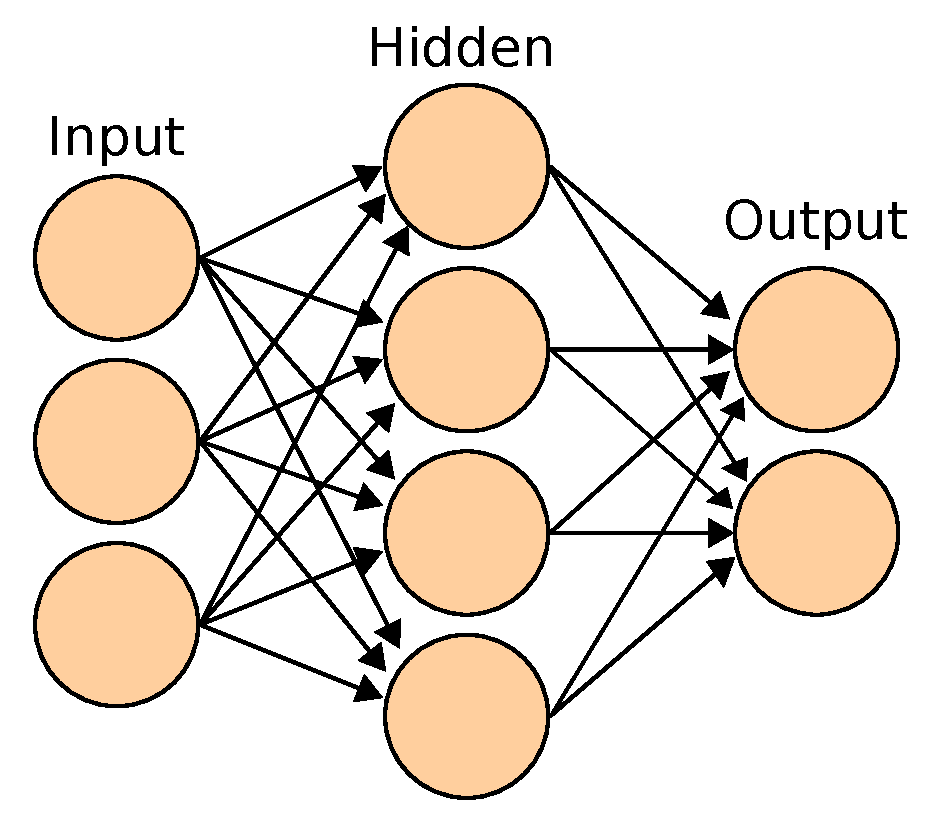
\includegraphics[width=4cm]{ANN.pdf}};
\end{tikzpicture}
\end{frame}

\subsection{}
\begin{frame}{Hebb a BAM}
\begin{itemize}
\item Hebbovské učení: {\em ``What fires together, wires together.''} \\
	$\Delta w_{ij} = \gamma x_i y_j \qquad W' = W + \vec x^T \vec y$
\item TODO: obrazek
\item {\bf Bidirectional Associative Memory (BAM):}
	Dvouvrstvá (a)synchronní rekurentní síť s obousměrnými synapsemi, neurony každý s každým
\item Váhová matice $W$, jedna iterace je $\vec x \cdot W = \vec y$
\item Atraktory jsou vlastní vektory, nechť odpovídají vzorům
\item Kapacita matice $W$ je omezená (crosstalk); \\
	pro ortogonální vektory $m \simeq 0.18 n$
\item Korelační matice; neortogonální vektory: pseudoinverzní matice
\end{itemize}
\end{frame}

\subsection{}
\begin{frame}{Konvergence BAM}
\begin{itemize}
\item Zkonverguje vyhodnocování BAM? \pause Ano! Ale proč?
\pause
\item Vstup do sítě by se měl blížit předchozímu vstupu
\item Energetická funkce $E(\vec x, \vec y) = -{1 \over 2}\vec x W \vec y^T$
\item Lze ukázat, že v každé iteraci energetická funkce klesne!
\pause
\item Počet hodnot energetické funkce je konečný
\item QED
\end{itemize}
\end{frame}

\subsection{}
\begin{frame}{Hopfieldova síť}
\begin{itemize}
\item TODO: obrazek
\item Jednovrstvá rekurentní síť, neurony každý s každým
\item Rozpoznávání vzorů (2D matice), optimalizační problémy
\item Učení: $w_{ij} = \sum_{s=1}^m x_i^s y_i^s\quad i \ne j$
\item Rozpoznávání: Iterace do ustálení
\item Pro nulovou diagonálu konverguje (důkaz energetickou funkcí)
\end{itemize}
\end{frame}

\subsection{}
\begin{frame}{Optimalizační úlohy}
\begin{itemize}
\item Hopfieldův model minimalizuje chybovou funkci
\item $\Rightarrow$ je to řešítko optimalizačního problému!
\item Vyjádříme-li jiný (lineární) optimalizační problém podle funkce a pak zpětně odvodíme váhy neuronů, máme optimalizovátko
\end{itemize}
\begin{block}{Multiflop}
\begin{itemize}
\item Na konci je aktivní právě jeden neuron
\item Chybová funkce $E = \sum_i (x_i-1)^2$
\item Problém $n$ věží, TSP
\end{itemize}
\end{block}
\end{frame}

\subsection{}
\begin{frame}{Stochastické učení}
\begin{itemize}
\item TODO: obrazek
\item Hopfieldův model na funkci $E$ provádí {\bf hillclimbing}
\item Vždy se hýbeme po svahu co nejstrměji
\item Funkce $E$ má lokální minima, z nich se nedostaneme
\item Řešení: Stochastické uhýbání ze svahu
\item Simulované žíhání (annealing): $p_{\Delta E} = {1 \over 1 + e^{\Delta E/T}}$
\item Aplikace na Hopfieldův model: Boltzmannův stroj
\end{itemize}
\end{frame}

\subsection{}
\begin{frame}{Otázky?}
\begin{center}
Příště: Samoorganizace v rámci ANN.
\end{center}
\end{frame}

\section{Evoluční algoritmy}

\subsection{}
\begin{frame}{Rekapitulace --- genetický algoritmus}
\begin{itemize}
\item Populace řešení (s určitou strukturou), ohodnocovací funkce
\item Máme populaci předchozí generace, vyrábíme novou generaci (dokud nenajdeme optimum).
\item Nová generace (dokud není plná) --- aplikuj genetické operátory:
\begin{itemize}
\item Vyber dva jedince z minulé populace (selekce)
\item Vyrob dva nové jedince (křížení)
\item Mírně jedince uprav (mutace)
\item Dvojici vlož do nové generace
\end{itemize}
\end{itemize}
\end{frame}

\subsection{}
\begin{frame}{Reprezentační schémata}
\begin{itemize}
\item Popisujme řešení jako binární řetězec
\item Schéma $S$ je slovo v abecedě 0, 1 a * (don't care)
\item Schéma $S$ reprezentuje množinu řešení
\item Řád schématu $o(S)$, definující délka $d(S)$, fitness $F(S)$
\vskip 3ex
\pause
\item {\bf Věta o schématech:} Schémata, která jsou krátká, nadprůměrná a malého řádu se v populaci exponenciálně množí
\item Důkaz: Vliv operátorů na atributy schémat
\item Tedy na kódování záleží!
\item Vzpomeňte si příště: Exploration vs. exploitation problem!
\end{itemize}
\end{frame}

\subsection{}
\begin{frame}{Evoluční a genetické programování}
\begin{itemize}
\item Model programu: Lispový funkcionální \\ model nebo konečný automat
\item Fitness: Přesnost výpočtu (ano/ne, \\ odchylka, \dots)
\item Mutace: Přidání/odebrání stavu nebo volání (prodloužení větve programu)
\item Crossover je problematický --- headless chicken!
\item Lineární genetické programování: Imperativní programování, trackování registrů, reprezentace pomocí bytecode
\item Meta-Optimizing Semantic Evolutionary Search (MOSES)
\end{itemize}
\begin{tikzpicture}[remember picture,overlay]
  \node [xshift=-4.5cm,yshift=-4.5cm,above right] at (current page.north east)
    {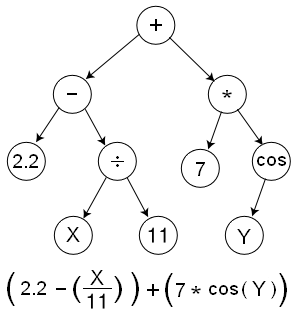
\includegraphics[width=4cm]{Genetic_Program_Tree.png}};
\end{tikzpicture}
\end{frame}

\subsection{}
\begin{frame}{Evoluční strategie}
\begin{itemize}
\item Evolvujeme nikoliv pouze jedince, ale i parametry evoluce
\item Jedinec je $(G,S)$, $S=(M,L,R)$
\item $M$ počet jedinců v populaci \\ $L$ počet potomků \\ $R$ počet rodičů (gang bang)
\item Křížení a mutace: Normální rozdělení, odchylky, rotace a průměr
\end{itemize}
\end{frame}

\subsection{}
\begin{frame}{Otázky?}
\begin{center}
Příště: Koevoluce a otevřená evoluce (brmlife). \\ Pravděpodobnostní model GA.
\end{center}
\end{frame}

\section{Datové struktury}

\subsection{}
\begin{frame}{Binární vyhledávací strom}
\begin{itemize}
\item Binární strom --- hrany pouze ``směrem dolů'', jeden kořen, každý uzel má nula (list) až dva syny
\item Vyhledávací strom --- vše v levém podstromu $\le n \le $ vše v pravém podstromu
\item Vyhledávání --- cesta z kořenu k uzlu
\item Vnitřní uzly --- data nebo navigace?
\item Chceme operace INSERT, DELETE
\item Naivně: INSERT do listu, rotace u DELETE
\pause
\item Jak vyrobit strom nad datasetem?
\vskip 3ex
\pause
\item Vyvážený strom --- hloubky podstromů se liší jenom málo
\item Ve vyváženém stromě trvá hledání $O(\log n)$
\item Jak vyrobit a udržovat vyvážený strom?
\end{itemize}
\begin{center}
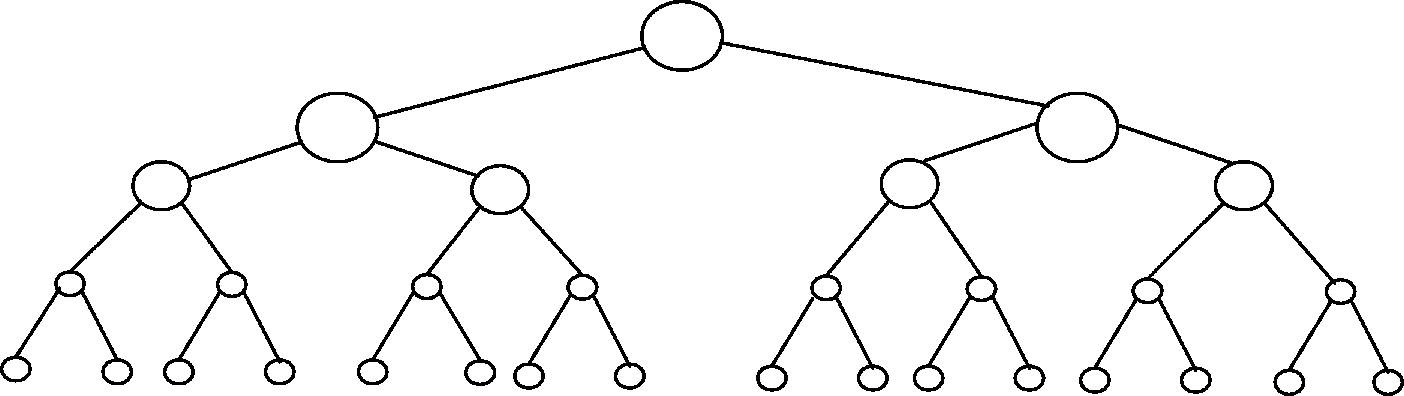
\includegraphics[width=8cm]{fullbintree.png}
\end{center}
\end{frame}

\subsection{}
\begin{frame}{Stromy rovnoměrně rozložených hodnot}
\begin{itemize}
\item Hodnoty jsou rovnoměrně rozložené (třeba hashe)
\item Je potřeba vůbec vyvažovat?
\end{itemize}
\end{frame}

\subsection{}
\begin{frame}{Splay stromy}
\begin{itemize}
\item Zavedeme operaci {\em splay} --- rotaci uzlu zevnitř stromu do kořene
\item FIND --- splay do kořene
\item INSERT --- do listu a splay
\item DELETE --- vymyslete!
\item Asymptoticky vyvážený strom
\end{itemize}
\end{frame}

\subsection{}
\begin{frame}{Červeno-černé stromy}
\begin{itemize}
\item Idea: některé vnitřní uzly červeně {\em obarvíme}; barvy opatrně střídáme
\item Kořen a virtuální listy jsou vždy černé \\
	Oba synové červeného uzlu jsou černí \\
	Každá cesta z kořene do listu má stejný počet černých
\item Je strom vyvážený? \pause Nejdelší cesta je max. dvojnásobek nejkratší
\item INSERT --- vložíme červený skorolist a opravíme obarvení
\item DELETE --- vyměníme za následující hodnotu, její původní uzel utrhneme a opravíme obarvení
\end{itemize}
\end{frame}

\subsection{}
\begin{frame}{AVL stromy}
\begin{itemize}
\item Idea: Každý uzel má balanční faktor; menší než -1 nebo větší než 1 je nutno opravit
\item INSERT --- vložíme, po cestě do kořene updatujeme a opravujeme balanční faktor
\item DELETE --- analogicky
\end{itemize}
\end{frame}

\subsection{}
\begin{frame}{Otázky?}
\begin{center}
Příště: B-stromy, haldy.
\end{center}
\end{frame}

\subsection{}
\begin{frame}{Děkuji vám}
\begin{center}
{\bf pasky@ucw.cz}

\vskip 6ex

Příště: Strojové učení podle zkušeností --- v umělé inteligenci obecně a~v~rámci adaptivních agentů. \\
	Neuronové sítě.
	Datové struktury.
\end{center}
\end{frame}

\end{document}
